\documentclass[aspectratio=169]{../latex_main/tntbeamer}  % you can pass all options of the beamer class, e.g., 'handout' or 'aspectratio=43'
\usepackage{dsfont}
\usepackage{bm}
\usepackage[english]{babel}
\usepackage[T1]{fontenc}
%\usepackage[utf8]{inputenc}
\usepackage{graphicx}
\graphicspath{ {./figures/} }
\usepackage{algorithm}
\usepackage[ruled,vlined,algo2e,linesnumbered]{algorithm2e}
\usepackage{hyperref}
\usepackage{booktabs}
\usepackage{mathtools}

\usepackage{amsmath,amssymb}

\DeclareMathOperator*{\argmax}{arg\,max}
\DeclareMathOperator*{\argmin}{arg\,min}

\usepackage{amsbsy}
\newcommand{\vect}[1]{\bm{#1}}
%\newcommand{\vect}[1]{\boldsymbol{#1}}

\usepackage{pgfplots}
\pgfplotsset{compat=1.16}
\usepackage{tikz}
\usetikzlibrary{trees} 
\usetikzlibrary{shapes.geometric}
\usetikzlibrary{positioning,shapes,shadows,arrows,calc,mindmap}
\usetikzlibrary{positioning,fadings,through}
\usetikzlibrary{decorations.pathreplacing}
\usetikzlibrary{intersections}
\pgfdeclarelayer{background}
\pgfdeclarelayer{foreground}
\pgfsetlayers{background,main,foreground}
\tikzstyle{activity}=[rectangle, draw=black, rounded corners, text centered, text width=8em]
\tikzstyle{data}=[rectangle, draw=black, text centered, text width=8em]
\tikzstyle{myarrow}=[->, thick, draw=black]

% Define the layers to draw the diagram
\pgfdeclarelayer{background}
\pgfdeclarelayer{foreground}
\pgfsetlayers{background,main,foreground}

% Requires XeLaTeX or LuaLaTeX
%\usepackage{unicode-math}

\usepackage{fontspec}
%\setsansfont{Arial}
\setsansfont{RotisSansSerifStd}[ 
Path=../latex_main/fonts/,
Extension = .otf,
UprightFont = *-Regular,  % or *-Light
BoldFont = *-ExtraBold,  % or *-Bold
ItalicFont = *-Italic
]
\setmonofont{Cascadia Mono}[
Scale=0.8
]

\renewcommand{\ttdefault}{Cascadia Mono}

% scale factor adapted; mathrm font added (Benjamin Spitschan @TNT, 2021-06-01)
%\setmathfont[Scale=1.05]{Libertinus Math}
%\setmathrm[Scale=1.05]{Libertinus Math}

% other available math fonts are (not exhaustive)
% Latin Modern Math
% XITS Math
% Libertinus Math
% Asana Math
% Fira Math
% TeX Gyre Pagella Math
% TeX Gyre Bonum Math
% TeX Gyre Schola Math
% TeX Gyre Termes Math

% Literature References
\newcommand{\lit}[2]{\href{#2}{\footnotesize\color{black!60}[#1]}}

%%% Beamer Customization
%----------------------------------------------------------------------
% (Don't) Show sections in frame header. Options: 'sections', 'sections light', empty
\setbeamertemplate{headline}{empty}

% Add header logo for normal frames
\setheaderimage{
	% 
\includegraphics[height=\logoheight]{figures/TNT_darkv4.pdf}
	
\includegraphics[height=\logoheight]{../latex_main/figures/Leibniz-AI-Academy_Logo}
	% 
\includegraphics[height=\logoheight]{figures/logo_tntluh.pdf}
}

% Header logo for title page
\settitleheaderimage{
	% 
\includegraphics[height=\logoheight]{figures/TNT_darkv4.pdf}
	
\includegraphics[height=\logoheight]{../latex_main/figures/Leibniz-AI-Academy_Logo}
	% 
\includegraphics[height=\logoheight]{figures/logo_tntluh.pdf}
}

% Title page: tntdefault 
\setbeamertemplate{title page}[tntdefault]  % or luhstyle
% Add optional title image here
%\addtitlepageimagedefault{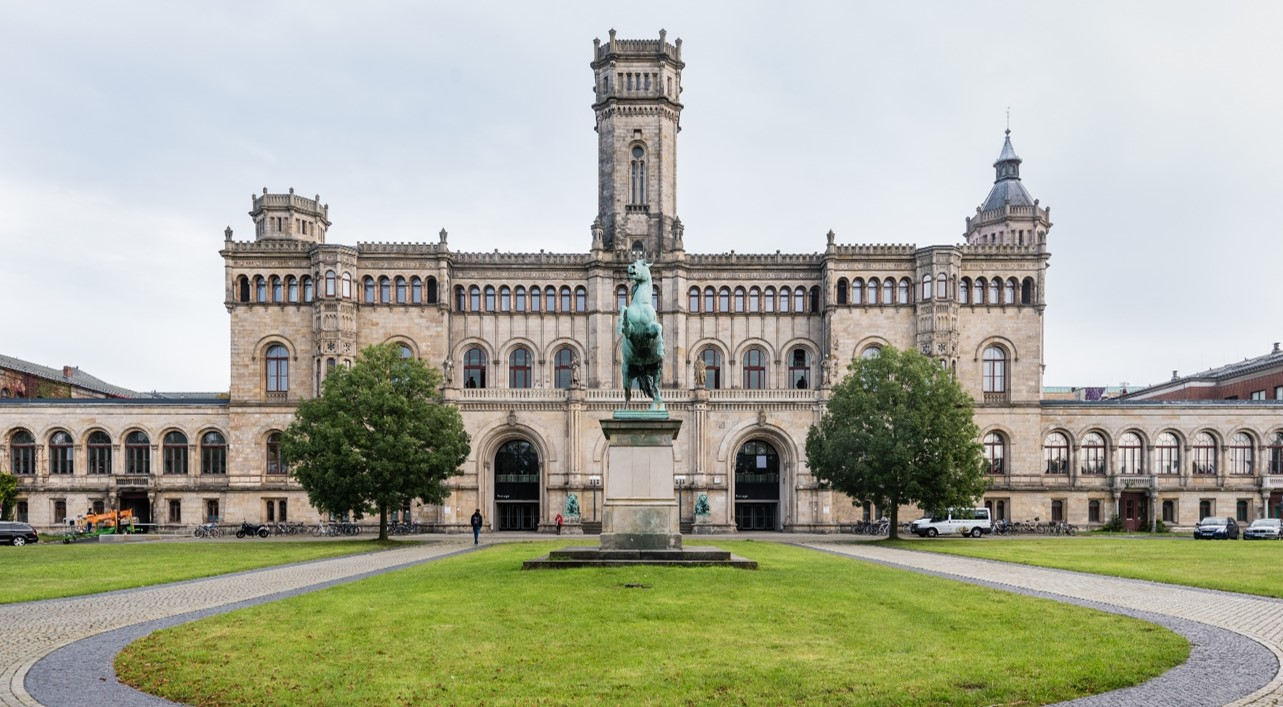
\includegraphics[width=0.65\textwidth]{figures/luh_default_presentation_title_image.jpg}}

% Title page: luhstyle
% \setbeamertemplate{title page}[luhstyle]
% % Add optional title image here
% \addtitlepageimage{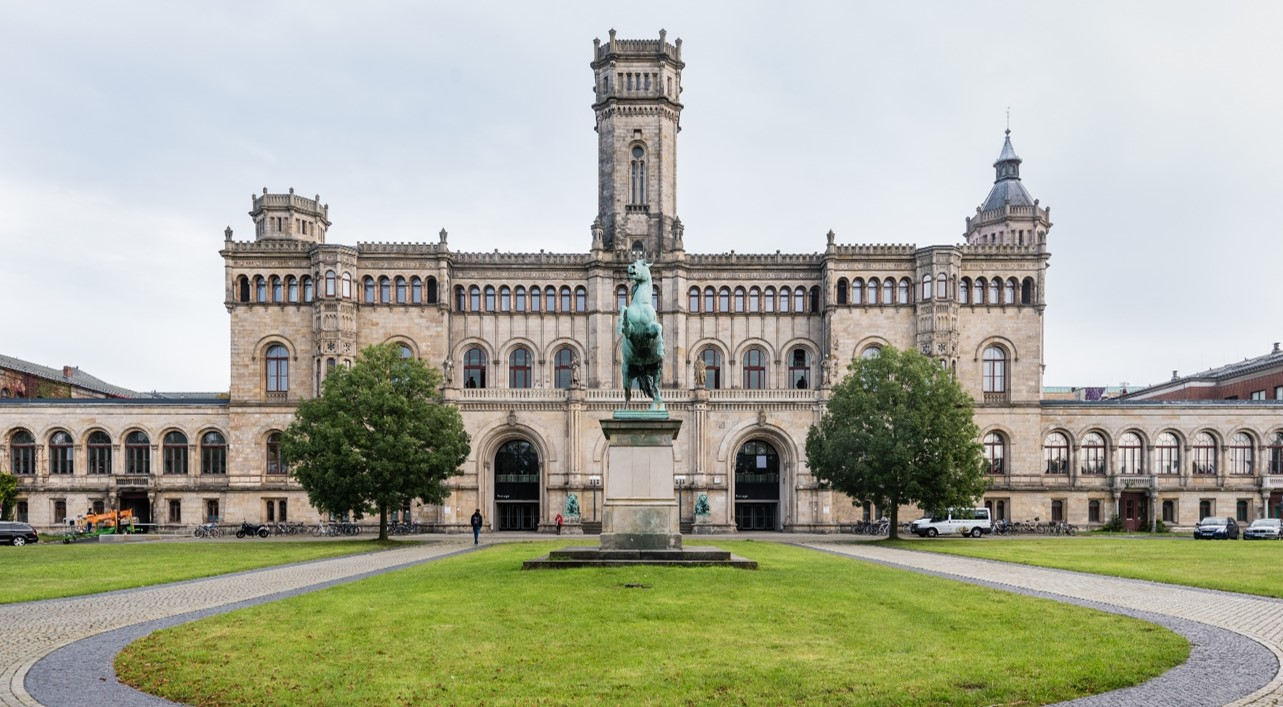
\includegraphics[width=0.75\textwidth]{figures/luh_default_presentation_title_image.jpg}}

\author[Abedjan \& Lindauer]{Ziawasch Abedjan \& \underline{Marius Lindauer}\\[1em]
	%
\includegraphics[height=\logoheight]{../latex_main/figures/luh_logo_rgb_0_80_155.pdf}\qquad
	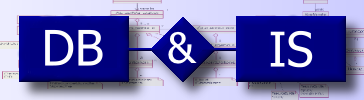
\includegraphics[height=\logoheight]{../latex_main/figures/DBIS_Kurzlogo.png}\qquad
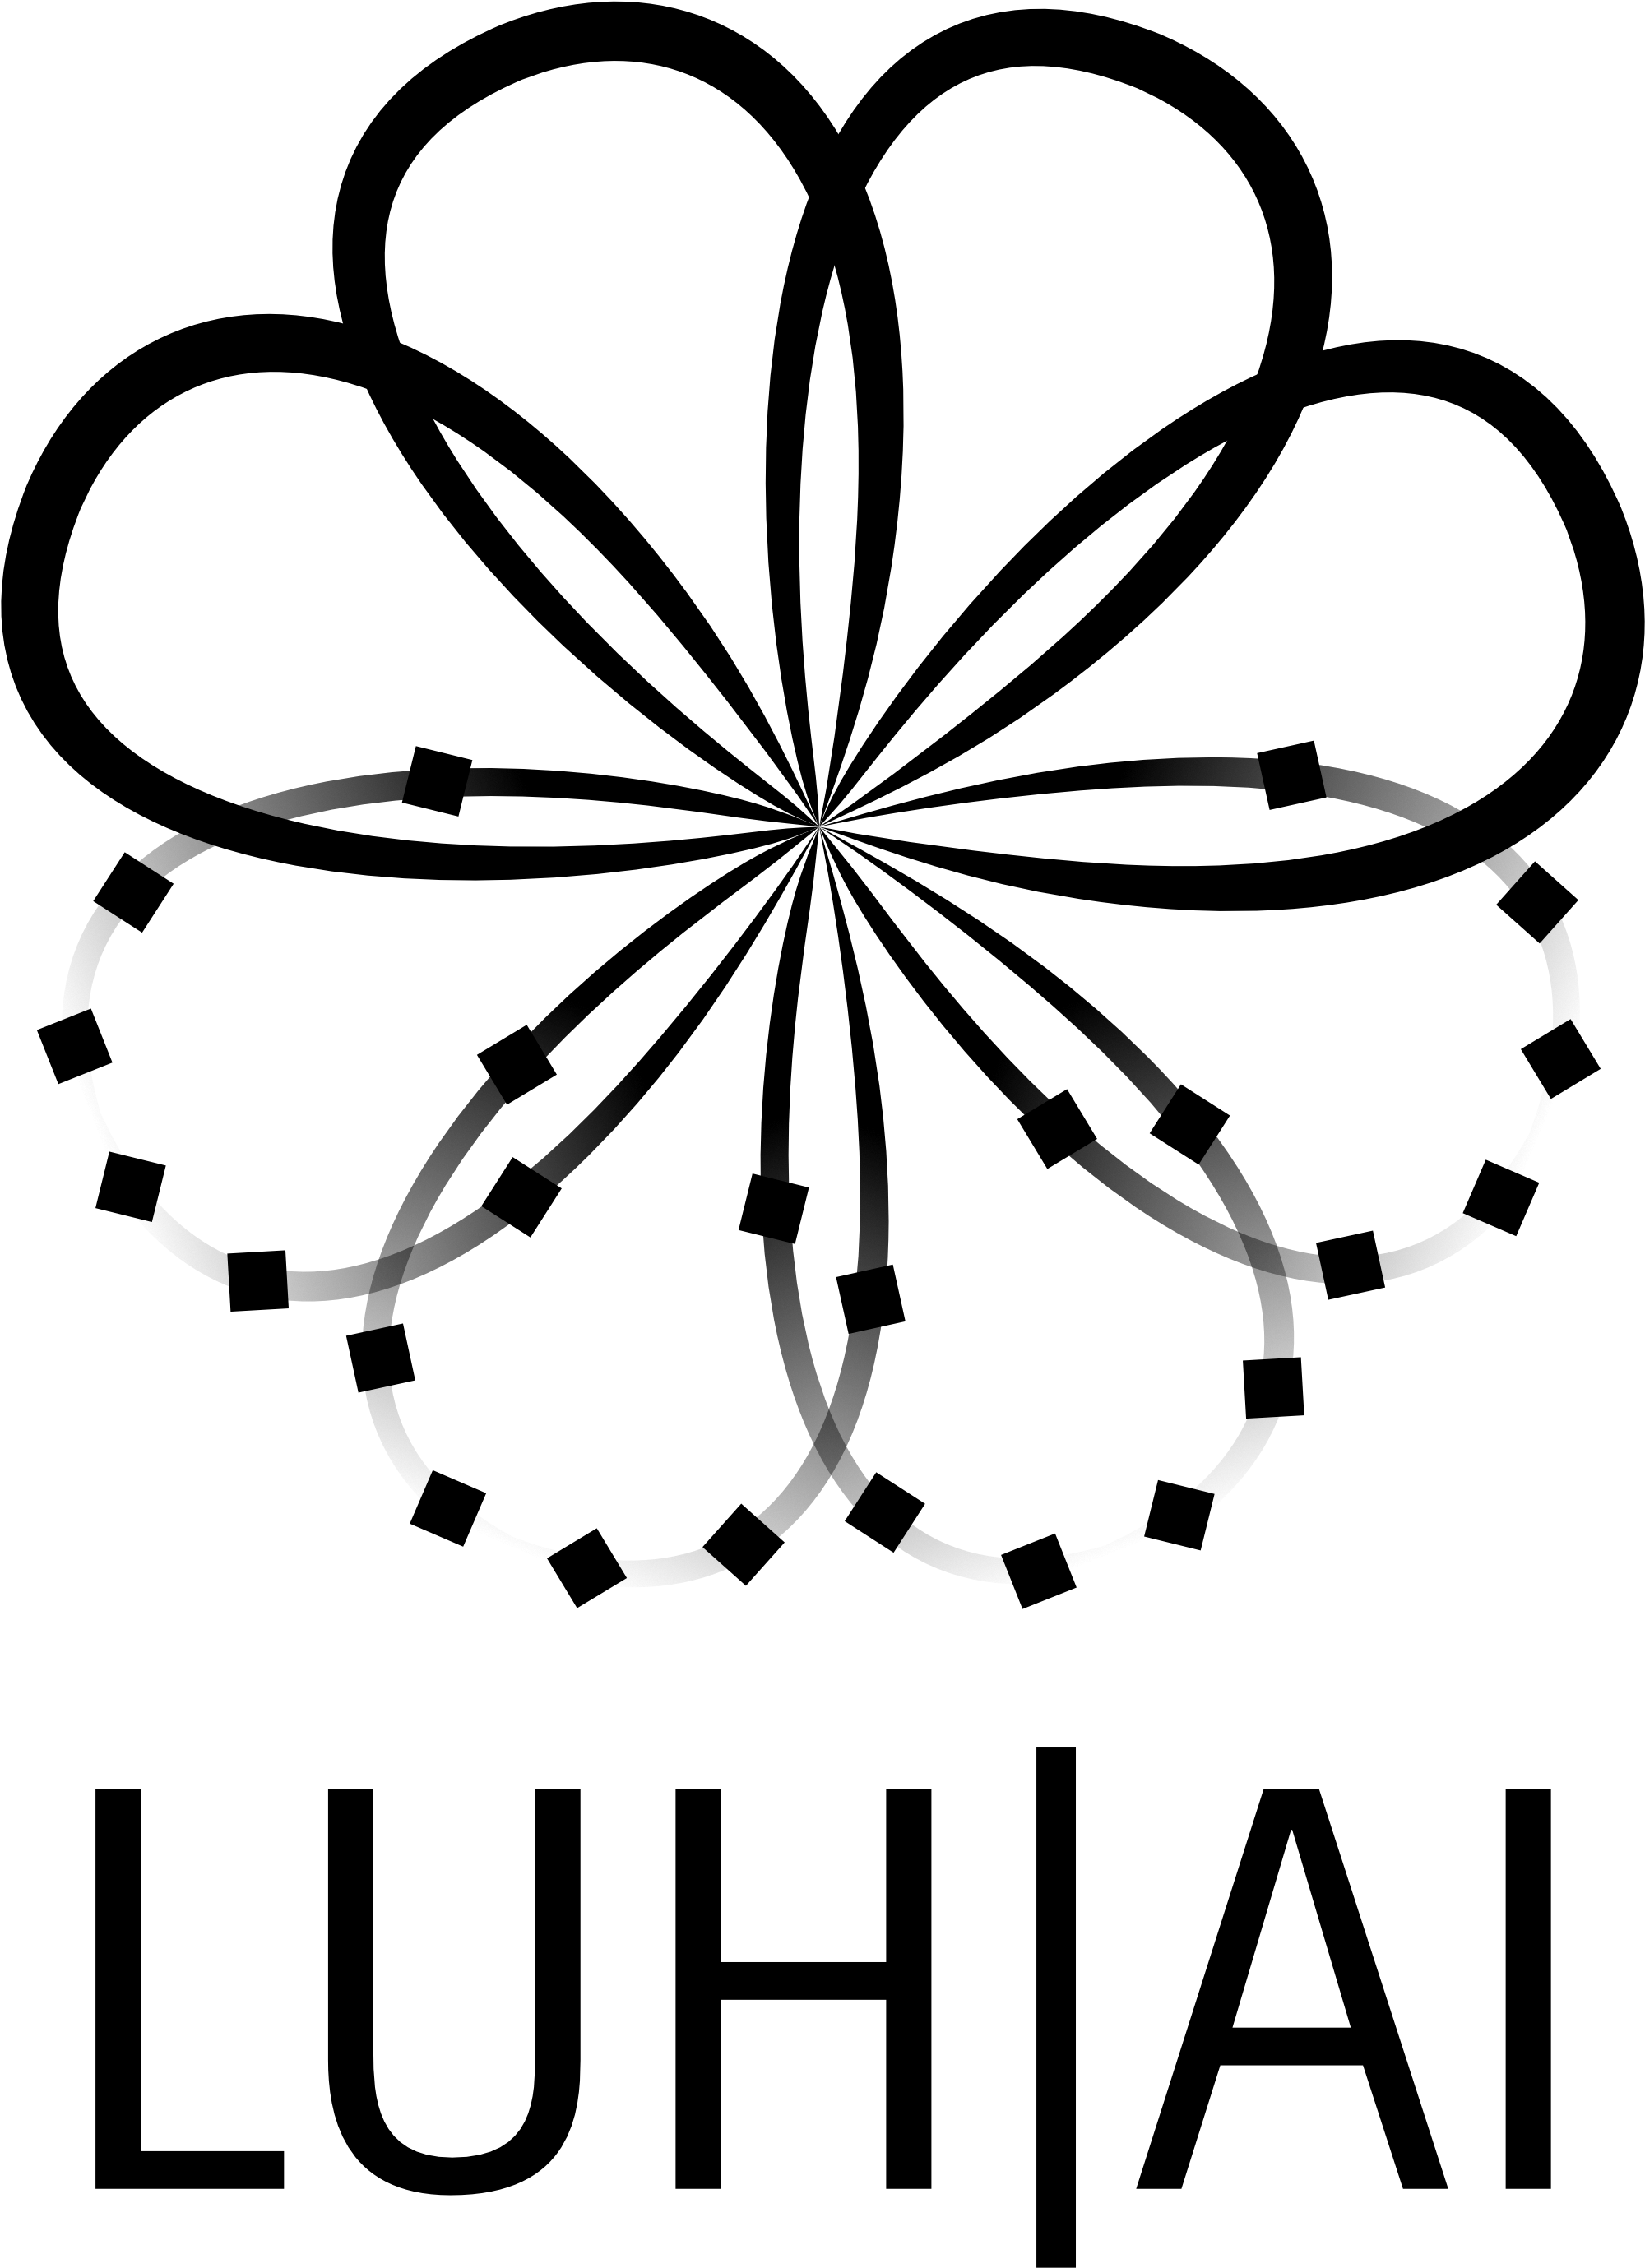
\includegraphics[height=\logoheight]{../latex_main/figures/logo_short_highres_black}\qquad

\includegraphics[height=\logoheight]{../latex_main/figures/Leibniz-AI-Academy_Logo}\qquad
%
\includegraphics[height=\logoheight]{../latex_main/figures/L3S.jpg}	
}
\date{\hspace{0.5em} {
\includegraphics[height=1.5em]{../latex_main/figures/Cc-by-nc-sa_icon.svg.png}}; extension of \href{https://ds100.org/fa21/}{[DS100]}
}


%%% Custom Packages
%----------------------------------------------------------------------
% Create dummy content
\usepackage{blindtext}

% Adds a frame with the current page layout. Just call \layout inside of a frame.
\usepackage{layout}


%%% Macros
%\renewcommand{\vec}[1]{\mathbf{#1}}
% \usepackage{bm}
%\let\vecb\bm

\title[Cleaning]{DS: Data Cleaning}
\subtitle{Cleaning}

\graphicspath{ {./figure/} }
%\institute{}


\begin{document}
	
	\maketitle

 \begin{frame}[c]{Motivation}

\begin{itemize}
    \item \textbf{Rules:}
    \begin{itemize}
        \item \textit{Example 1:} The city determines the state
        \begin{itemize}
            \item (t4 and t6 violate this rule)
        \end{itemize}
        \item \textit{Example 2:} Among employees having the same role, salaries in NYC should be higher
        \begin{itemize}
            \item (t5 and t6 violate this rule)
        \end{itemize}
    \end{itemize}
    \item Traditional methods apply rules one by one
\end{itemize}

\centering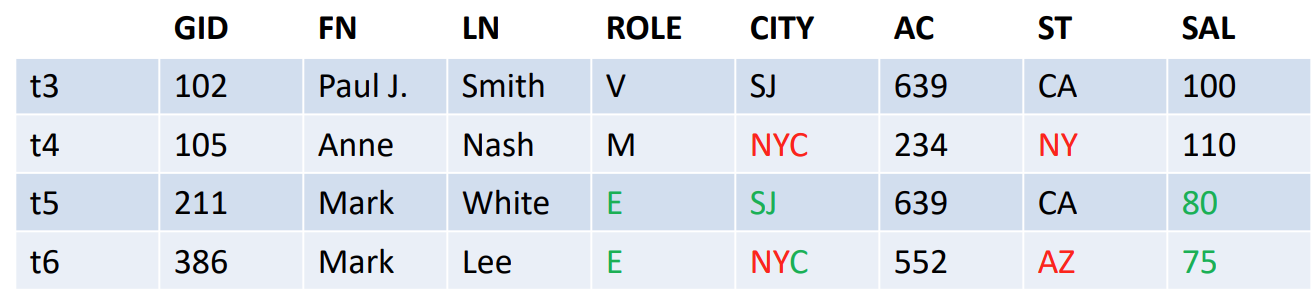
\includegraphics[width=0.8\textwidth]{figure/bild18_table}

\end{frame}

\begin{frame}[c]{Goal/Problem}

\begin{itemize}
    \item Correct violations for different types of constraints with desirable repairs
    \item $\leadsto$ {Desirability} depends on a cost model such as minimizing the number of changes
    \item How can we compile heterogeneous rules into the same language and efficiently apply them holistically together?
\end{itemize}

\end{frame}

\begin{frame}[c]{Denial Constraints}

\begin{itemize}
    \item The method accepts \textbf{Denial Constraints (DCs)} as input
    \item DCs are a declarative specification of the quality rules
\end{itemize}

\centering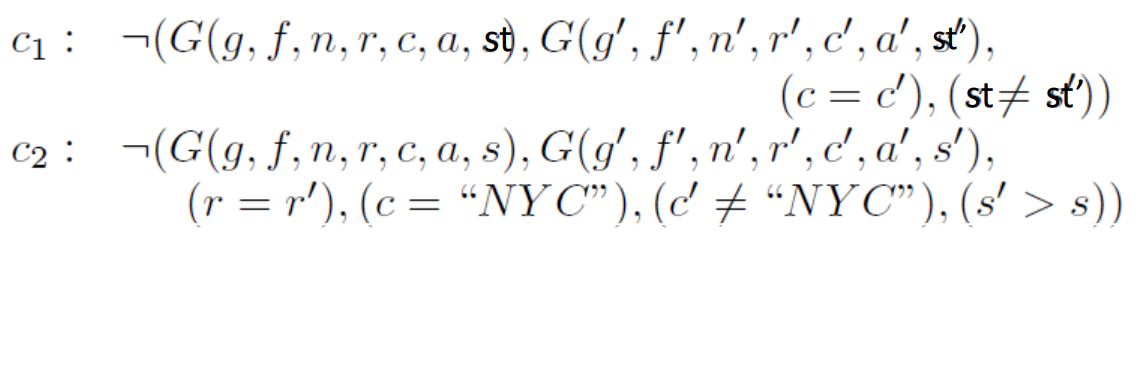
\includegraphics[width=0.8\textwidth]{figure/bild19_constraints}

\vspace{-2cm}

\begin{itemize}
    \item \textbf{Example Data:}
    \end{itemize}
    \begin{center}
        \begin{tabular}{|c|c|c|c|c|c|c|c|}
            \hline
            GID & FN & LN & ROLE & CITY & AC & ST & SAL \\
            \hline
            t3 & 102 & Paul J. Smith & V & SJ & 639 & CA & 100 \\
            t4 & 105 & Anne Nash & M & NYC & 234 & NY & 110 \\
            t5 & 211 & Mark White & E & SJ & 639 & CA & 80 \\
            t6 & 386 & Mark Lee & E & NYC & 552 & AZ & 75 \\
            \hline
        \end{tabular}
    \end{center}

\end{frame}

\begin{frame}[c]{System Overview}

\begin{itemize}
    \item \textbf{Conflict Hypergraph (CH)}: Encodes constraint violations
    \item \textbf{Repair Context (RC)}: Encodes violation repairs
\end{itemize}

\centering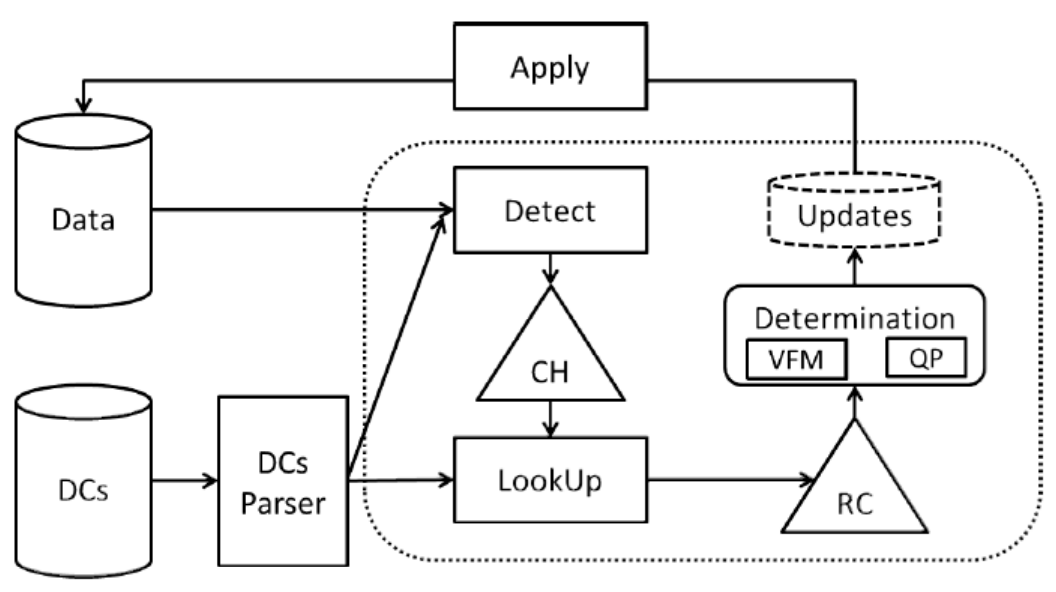
\includegraphics[width=0.6\textwidth]{figure/bild20_systems}

\end{frame}

\begin{frame}[c]{Violations Representation: Conflict Hypergraph}

\begin{itemize}
    \item The nodes represent the violating cells
    \item The edges link cells involved in the same violation
\end{itemize}

    \centering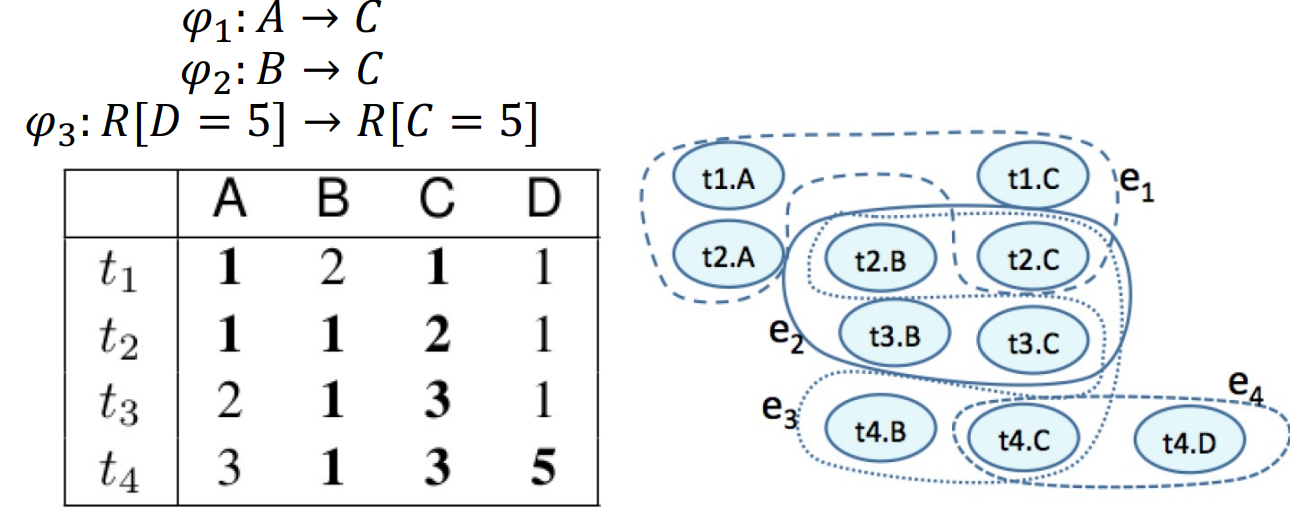
\includegraphics[width=0.9\textwidth]{figure/bild21_graphs}

\end{frame}

\begin{frame}[c]{Fixing Violation Holistically: Repair Context}

\begin{itemize}
    \item Start from cells identified by the minimum vertex cover as likely to be changed, e.g., \( t2[C] \)
\end{itemize}
    
    \begin{columns}
    
        \column{0.6\textwidth}

    \begin{enumerate}
        \item Start with \( t2[C] \) in queue; involved in 3 hyper-edges
        \item \textbf{Consider \( e_1 \):}
        \begin{itemize}
            \item Add repair \( t2[C] = t1[C] \); Add \( t1[C] \) to queue
        \end{itemize}
        \item \textbf{Consider \( e_2 \):}
        \begin{itemize}
            \item Add repair \( t2[C] = t3[C] \); Add \( t3[C] \) to queue
        \end{itemize}
        \item \textbf{Consider \( e_3 \):}
        \begin{itemize}
            \item Add repair \( t2[C] = t4[C] \); Add \( t4[C] \)
        \end{itemize}
        \item \textbf{Considering \( e_4 \):}
        \begin{itemize}
            \item Add repair \( t4[C] = 5 \)
        \end{itemize}
    \end{enumerate}
    
        \column{0.4\textwidth}
    
        \centering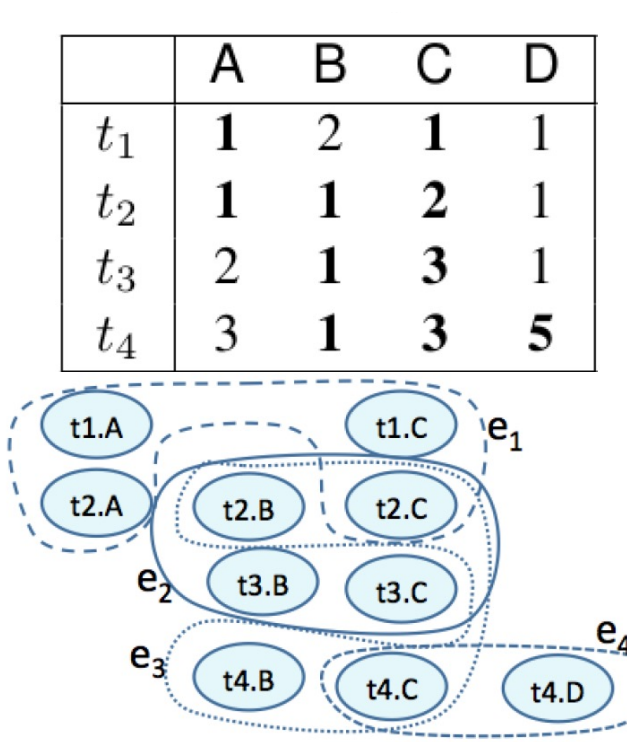
\includegraphics[width=.8\textwidth]{figure/bild22_graphs2}
    
    \end{columns}


\end{frame}

\end{document}